\paragraph{}En este proceso, el usuario administrador de centro puede crear,
consultar, modificar o borrar asignaciones de usuarios asesores a alumnos de la
aplicación.

\paragraph{}La figura \ref{diagramaNivel4-GestionarAsignacion}
muestra el nivel de abstracción 4: Gestionar asignación de asesores a alumnos.

  \begin{figure}[!ht]
    \begin{center}
      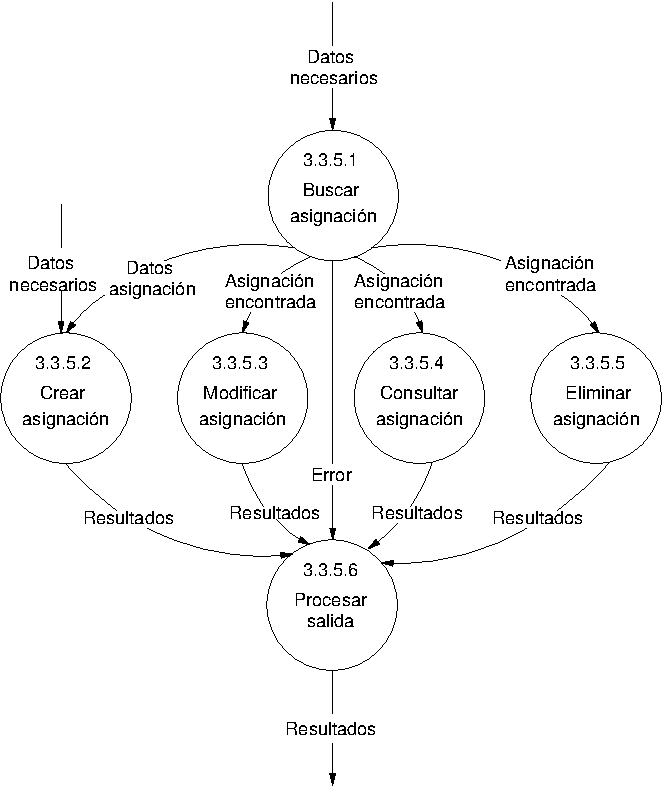
\includegraphics[]{08.Analisis_Funcional/8.2.DFDs/Niveles/Nivel4/AdministradorCentro/GestionarAsignacion/Diagramas/nivel4-GestionarAsignacion.pdf}
      \caption{Nivel de abstracción 4: Gestionar asignación de asesores a alumnos.}
      \label{diagramaNivel4-GestionarAsignacion}
    \end{center}
  \end{figure}
